\documentclass[a4paper, 12pt, twoside]{article}

\usepackage[francais]{babel}
\usepackage[utf8]{inputenc}
\usepackage{lmodern}
\usepackage[T1]{fontenc}
\usepackage{layout}

\usepackage{fancyhdr}
\usepackage{soul}
\usepackage{url}
\usepackage{color}
\usepackage{graphicx}
\usepackage{array}
\usepackage{geometry}
\usepackage{float}


\title{\hrule \vspace{1cm} Dossier de Conception : PicExplorer}
\author{\textsc{Lanvin} Elyan - \textsc{Marcais} Thomas\\ \textsc{Ramolet} Arthur - \textsc{Guenver} Loïc\\ \textsc{Aydin} Emre - \textsc{Foucault} Antoine}
\date{\today}

\begin{document}

%Définition du style des bords de page
\pagestyle{fancy}
\lhead{}
\chead{}
\rhead{\leftmark}
\lfoot{Groupe C}
\cfoot{}
\rfoot{Page \thepage}

%Titre
\clearpage
\thispagestyle{empty}

\maketitle
\begin{center}
 \copyright 2014 Groupe C - Tous droits reservés\\
\end{center}
\vspace{1cm}
\hrule
\thispagestyle{empty}

\newpage

%Sommaire
\renewcommand{\contentsname}{Sommaire}
\tableofcontents
\newpage

%Corps
\section{Introduction}

\subsection{Présentation du document}

Ce document est le dossier de conception du projet “CrosSPI”. Il a pour objectif de décrire précisément l’architecture du projet ainsi que les outils et technologies utilisés pour sa mise en application.
\smallbreak
Ce document fait référence au cahier des charges du projet qui définit les besoins du client, les fonctionnalités nécessaires et les contraintes imposées du projet.

\subsection{Contexte}

Ce document explicite l’architecture, les renseignements techniques ainsi que les contraintes à prendre en compte lors du développement de l’application.
\smallbreak
Il a pour but de définir le produit et de détailler sa conception afin qu’il soit à la fois conforme à la conception décidée par le chef de projet et cohérente par rapport aux attentes du client.

\subsection{Portée du document}

Il est destiné :

\begin{itemize}\setlength{\itemsep}{3mm}
 \item Aux professeurs du département informatique nous évaluant sur ce projet.
 \item A l'équipe du projet lors de la phase d'implémentation.
\end{itemize}

\smallbreak
Il servira de base :

\begin{itemize}\setlength{\itemsep}{3mm}
 \item A l'évaluation du produit final.
 \item Au développement des différents produits.
\end{itemize}

\section{Présentation du projet}

\subsection{Contexte}

Il se déroulera dans le cadre d’un projet tuteuré lors du semestre 6 de 3ème année de licence SPI.
\smallbreak
Il est réalisé par un groupe de 6 étudiants dont un chef de projet en charge de la coordination des membres du groupe et du travail ainsi que d’un documentaliste chargé de mettre en forme les différents livrables écrits à rendre.

\subsection{Objectifs}

Ce projet doit aboutir à la création d’une application dédiée au jeu de Picross, sur PC et pour tout système d’exploitation, destinée à tout type d’utilisateur.
\smallbreak
Cette application sera divisée en deux parties majeures :
\smallbreak
\begin{itemize}\setlength{\itemsep}{1mm}
 \item Edition de grilles de Picross avec importation/exportation de grille.
 \item Jeu de Picross avec sauvegarde/chargement de parties et aide à la résolution.
\end{itemize}

\subsection{Critères d'acceptabilité du produit}

L’application doit répondre aux critères suivants :
\smallbreak
\begin{itemize}\setlength{\itemsep}{1mm}
 \item Validation du produit via une série de tests réalisés par notre groupe. 
 \item Respect des contraintes client (choix technologiques, fonctionnalités de l'application).
\end{itemize}


\section{Environnement et outils de développement}

\subsection{Technologies utilisées pour l'implémentation}

\ul{Ruby (version 1.9.3)}\newline

Ruby est un langage de programmation libre et tout-objet (chaque élément est lié à un objet) dont les fichiers, en .rb,  sont interprétés. Il a été créé en 1995 par Yukihiro Matsumoto. Nous utiliserons ce langage pour l’implémentation de l’application, il sera la base du programme. Dans notre projet, nous travaillons avec sa version 1.9.3 afin d’assurer la compatibilité avec les ordinateurs de l’Université et Hop3x, ce qui est une des contraintes techniques imposées par le client.\\

\ul{Librairie graphique Gtk 2}\newline

The Gimp ToolKit (GTK) est un ensemble de librairies logicielles contenant des fonctions qui permettent la réalisation d’interfaces graphiques pour différentes langages de programmation tels que Ruby, Java, C++ ou encore PHP. De même que pour Ruby, nous utilisons la version 2 de GTK, antérieure à la plus récente, afin d’assurer la compatibilité avec les postes de l’Université.\\

\ul{SQLite}\newline

SQLite est une librairie écrite en C proposant un moteur de gestion de base de données relationnelle accessible par le langage SQL. A la différence d’un SGBD “classique” (architecture client-serveur), SQLite est directement intégré, en local, au programme. Dans le cadre du projet, il nous servira à enregistrer nos données après extinction du programme et à les récupérer lors de son démarrage.\\

\subsection{Environnements de développements}

\ul{IDE Hop3x}\newline

Hop3x est un environnement de développement créé en Java et appartenant à l’Université du Maine. Il permet d’éditer et de compiler des programmes en C, Ruby ou encore Java et de sauvegarder ces projets en ligne.\\

\ul{GitHub}\newline

GitHub est une plate-forme de gestion de versions basée sur Git permettant de gérer les différentes versions des codes sources d’un logiciel au cours de son développement. Par exemple il permet d’ajouter des fonctionnalités en parallèle du projet jusqu’à sa version finale.\\

\subsection{Autres}

\ul{RubyDoc}\newline

Le Ruby Document Format est un langage de balisage que l’on peut mélanger avec le code source Ruby. Il permet de générer une documentation propre en fonction du code balisée.\\

\newpage
\section{Architecture du projet}

\subsection{Conception générale du projet}

Afin de mieux structurer notre code et d’assurer une meilleure portabilité, nous avons choisi d’appliquer le design pattern Modèle Vue-Contrôleur. Son fonctionnement globale est détaillée dans le schéma ci-dessous :
\medbreak
\begin{figure}[H]
  \center
  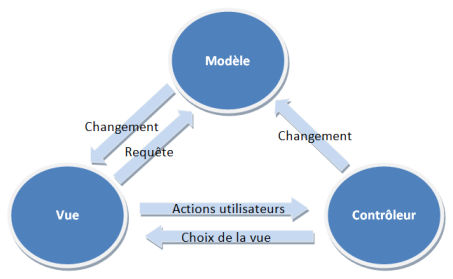
\includegraphics[scale=0.5]{mvc.png}
  \caption{Fonctionnement du modèle MVC}
  \label{MVC}
\end{figure}
\medbreak
A chaque nouvelle interface, la classe Picross (voir Diagramme de classe ci-dessous) chargera le trio MVC concret associé. Par exemple pourl’interface “Editeur”, nous aurons VueEditeur, ModeleEditeur et ControleurEditeur.

\newpage
\subsection{Diagramme de classe}

\begin{figure}[H]
  \center
  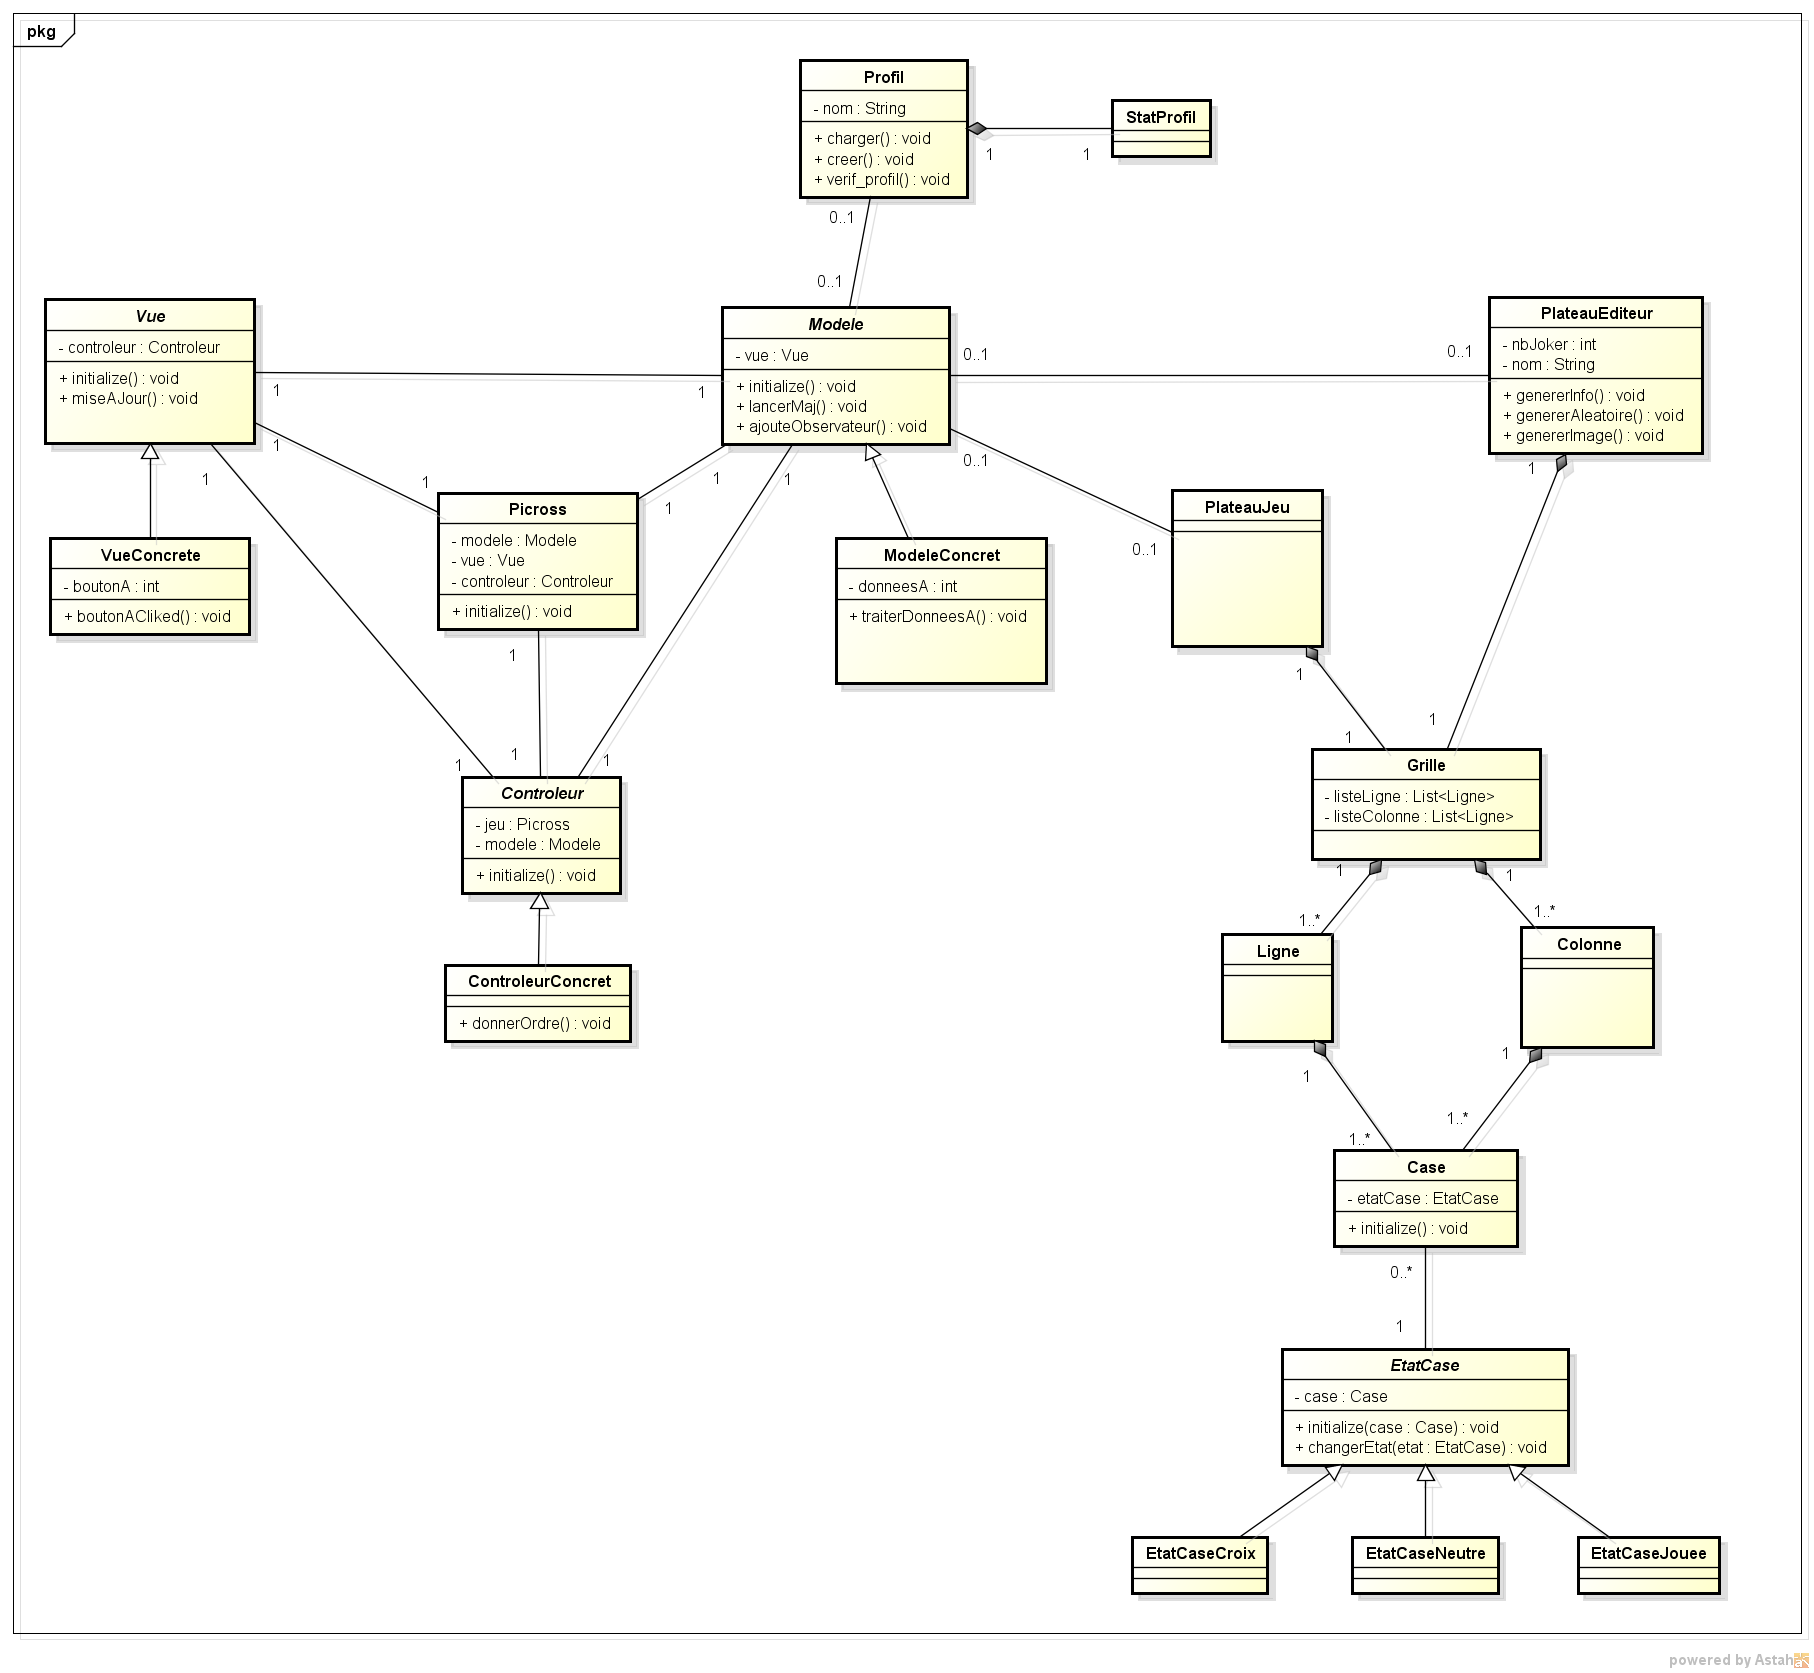
\includegraphics[scale=0.3]{diagrammeClasse.png}
  \caption{Diagramme de classe de l'application}
  \label{diagClasse}
\end{figure}

\newpage
\subsection{Schéma de navigation}

Ci-dessous, le schéma de navigation de l’application, c’est-à-dire la représentation par un diagramme des liens d’accès entre les différentes interfaces de l’application :

\bigbreak

\begin{figure}[H]
  \center
  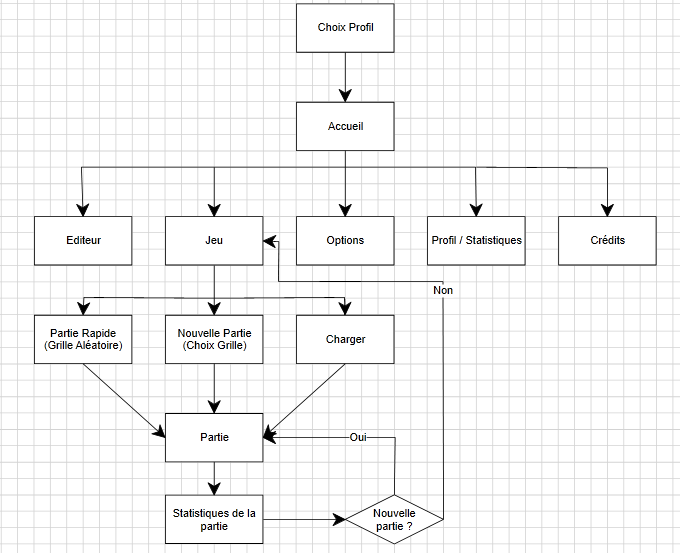
\includegraphics[scale=0.8]{schema_navigation.png}
  \caption{Schéma de navigation de l'application}
  \label{schema_navig}
\end{figure}

\newpage
\subsection{Utilisation de SQLite et modèle relationnel}

Au lieu  d’utiliser la sérialisation via YAML pour la persistance des données, nous avons préféré opter pour une base de données locale SQLite. Le modèle relationnel prévu sera le suivant :

\bigbreak

\begin{figure}[H]
  \center
  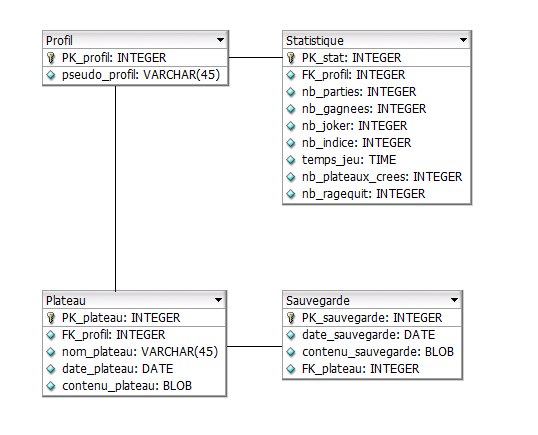
\includegraphics[scale=1]{MEA.png}
  \caption{Modèle Entité-Association de l'application}
  \label{mea}
\end{figure}

\newpage
\section{Spécifications des interfaces}

\subsection{Accueil}

\begin{figure}[H]
  \center
  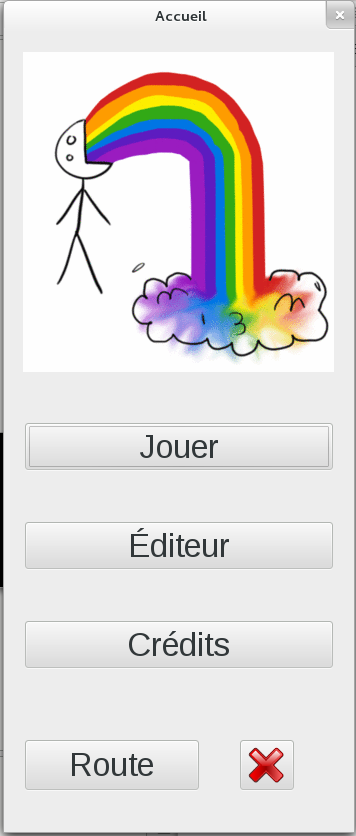
\includegraphics[scale=0.6]{accueil.png}
  \label{accueil}
\end{figure}
\newpage
\subsection{Editeur de grille}

\begin{figure}[H]
  \center
  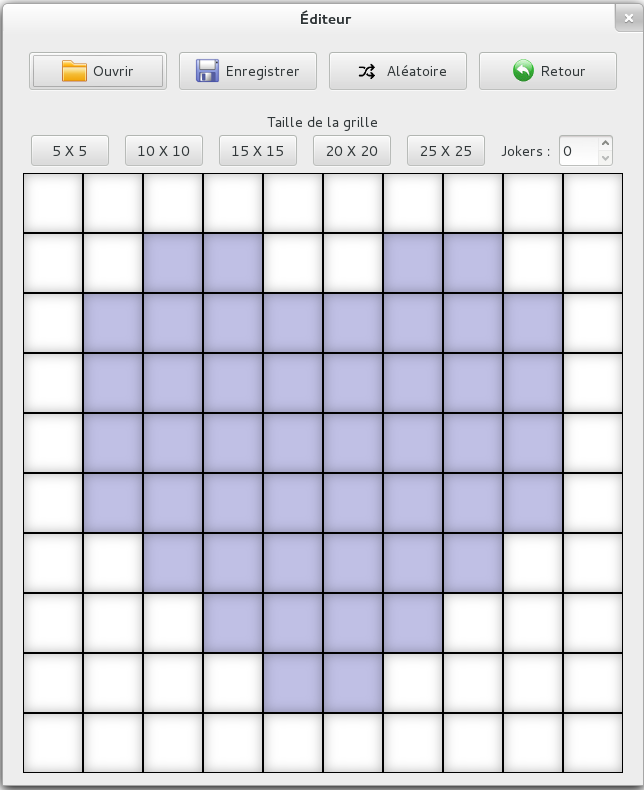
\includegraphics[scale=0.6]{editeur.png}

  \label{editeur}
\end{figure}
\newpage
\subsection{Jeu}

\begin{figure}[H]
  \center
  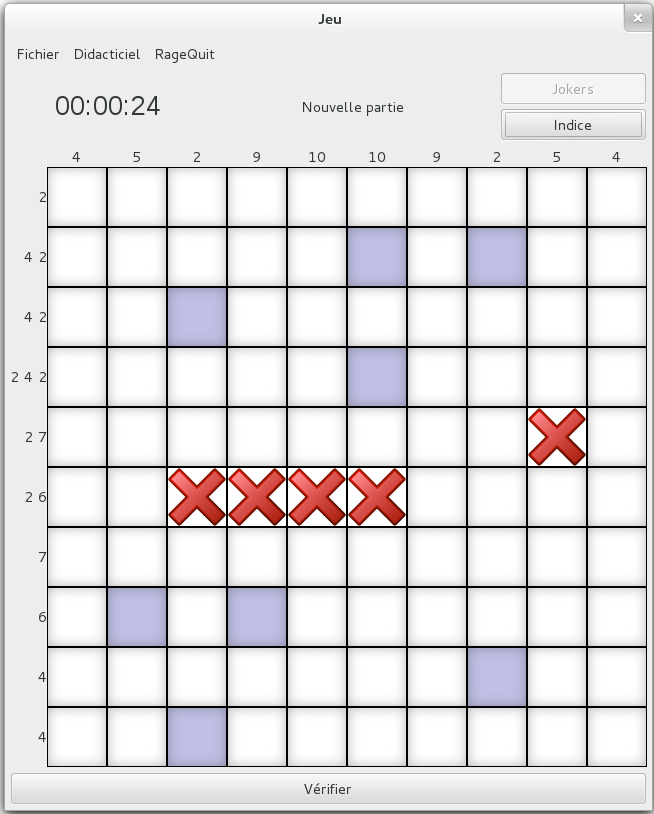
\includegraphics[scale=0.6]{jeu.png}
  \label{jeu}
\end{figure}
\newpage
\subsection{Statistiques}

\begin{figure}[H]
  \center
  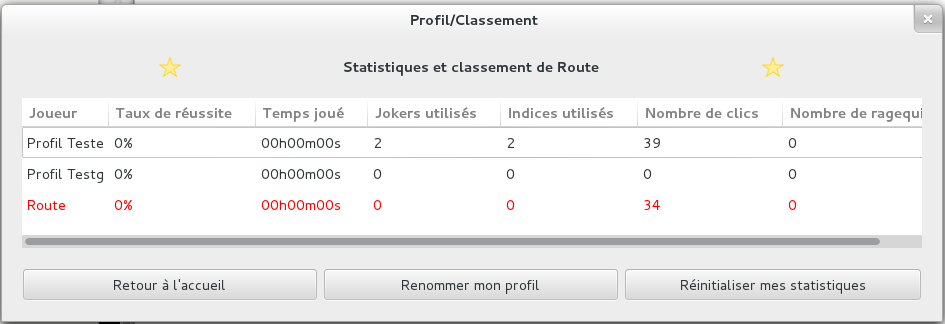
\includegraphics[scale=0.4]{stats.png}
  \label{stats}
\end{figure}

\bigbreak

\subsection{Connexion}

\begin{figure}[H]
  \center
  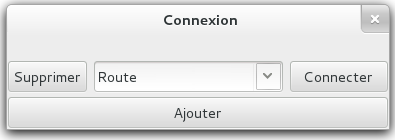
\includegraphics[scale=0.8]{connexion.png}
  \label{connexion}
\end{figure}

\end{document}
